\newcommand{\ClassPath}{../VIU_TFM_LaTeX_template}
\documentclass{\ClassPath/viu-tfm-template}
\usepackage{multicol}

\definecolor{maincolor}{HTML}{f25416}

%--------------------------------------------------------------------------
% Definiciones necesarias Modifica con tus datos
%--------------------------------------------------------------------------
\def\nombre{Gómez Olivencia, Rubén}
\def\dni{78910013-A}
\def\titulo{Introducción a AWS}
\def\titulacion{Máster Universitario en Desarrollo de Aplicaciones y Servicios Web}
\def\curso{2022-2023}

%Los siguientes son opcionales: si no se ponen, la portada cambia un poco. Ideal para escribir artículos/trabajos cortos
\def\dirige{}
\def\convocatoria{}
\def\asignatura{Computación en la nube}


% importar fichero de Bibliografía
%\addbibresource{Actividad_1.bib}

\begin{document}
    \graphicspath{{../VIU_TFM_LaTeX_template/}}

    \coverpage

    \tableofcontents

\chapter{Introducción}

A la hora de poner un proyecto en producción es aconsejable conocer las distintas alternativas que podemos utilizar para llevarlo a cabo. Hasta hace no muchos años, lo habitual era realizar el despliegue en un servidor propio situado en algún CPD.

Debido a las dificultades que puede suponer el gestionar unos servidores propios, junto con el no poder realizar el escalado del proyecto de manera sencilla, ha supuesto la mayor demanda de utilizar sistemas \textit{cloud} que facilitan dicha labor.

Es por eso que a lo largo de este documento se va a realizar una introducción a \textbf{AWS} (Amazon Web Services) junto con el despliegue de la aplicación \href{https://flarum.org/}{Flarum} en un servidor creado en este \textit{cloud}


\chapter{Base de datos RDS}
Para la aplicación se va a necesitar una base de datos, por lo que va a ser lo primero que se va a desplegar.

AWS permite realizar el despliegue de distintos gestores de bases de datos a través de su servicio \textbf{RDS} (\textit{Relational Database Service}). En este caso se va a desplegar un RDS de MySQL 5.X con las siguientes características:

\begin{itemize}
    \item RDS de tipo db.t3.micro
    \item Almacenamiento 20Gib SSD de uso general (gp2).
    \item MultiA-Z no.
    \item Cifrado en reposo habilitado.
    \item Configurar los backups automáticos para que se ejecuten a las 3:00 UTC con período de retención de 10
    días.
    \item Configurar la ventana de mantenimiento de actualizaciones a las 4:00 UTC.
\end{itemize}

A continuación parte de la configuración realizada durante la creación de la misma:

\begin{center}
    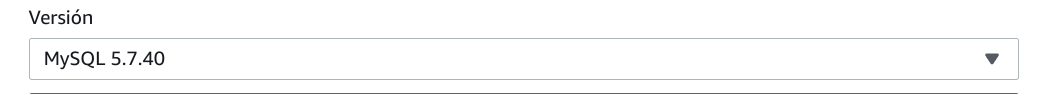
\includegraphics[width=0.8\linewidth]{img/db1.png}
    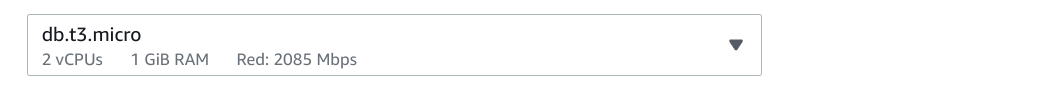
\includegraphics[width=0.8\linewidth]{img/db2.png}
    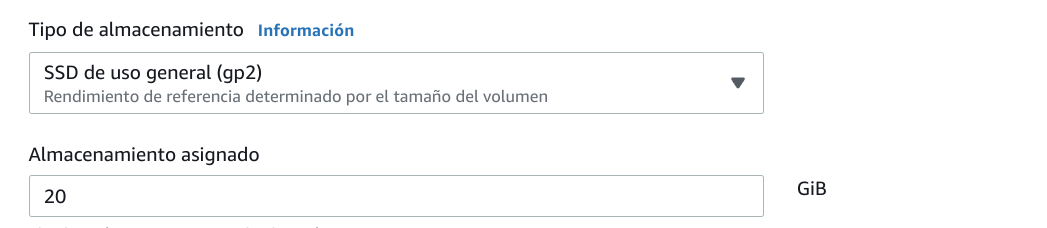
\includegraphics[width=0.8\linewidth]{img/db3.png}
    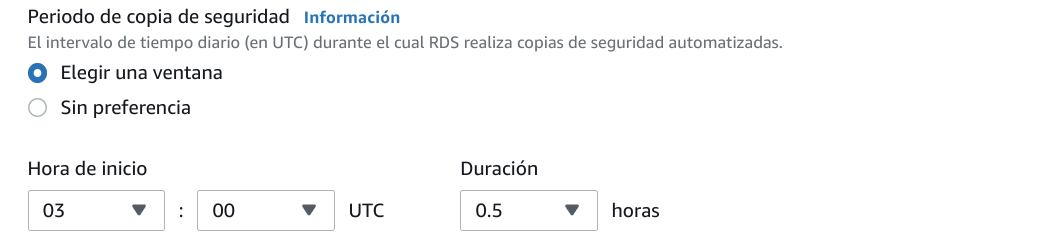
\includegraphics[width=0.8\linewidth]{img/db4.png}
    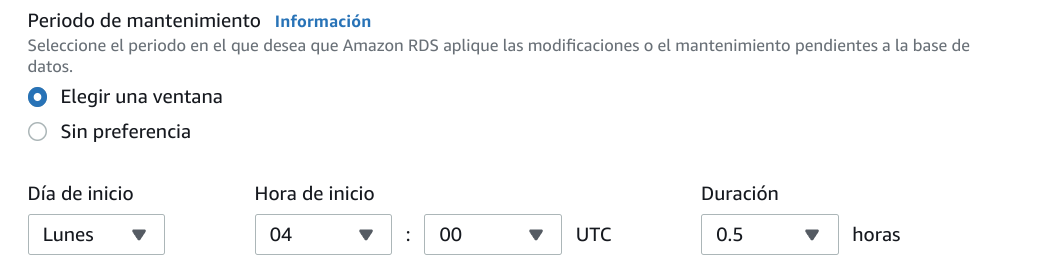
\includegraphics[width=0.8\linewidth]{img/db5.png}
\end{center}


A la hora de crear la base de datos se ha elegido crear una contraseña automática, por lo que es importante visualizarla y copiarla, ya que de no ser así, habría que volver a crear la base de datos.

% admin  -    hVviJyUovlhwRrRSrrRd

Hay que tener especial cuidado con el acceso al puerto 3306, por lo que se ha creado un grupo de seguridad propio que limitará únicamente el acceso a la IP pública de mi conexión y desde la IP de la instancia que se comentará posteriormente.

\begin{center}
    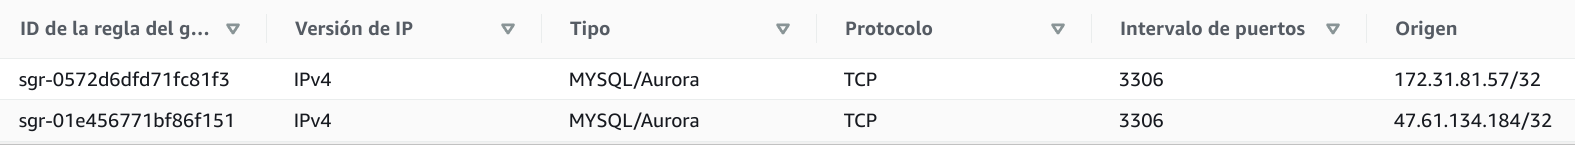
\includegraphics[frame,width=\linewidth]{img/db-reglas.png}
\end{center}

No se ha añadido la regla del tráfico saliente, ya que mantenemos la regla creada por defecto que habilita todo el tráfico que sale de la base de datos. Para mayor seguridad, podríamos hacer lo mismo, pero no es necesario.


De esta manera, a partir de ahora se podrá acceder al puerto 3306 con los credenciales que nos ha creado el asistente y podremos realizar la conexión utilizando el host \textbf{database-1.c92nioexause.us-east-1.rds.amazonaws.com}

Para asegurar que tenemos acceso, se utiliza el programa \href{https://dbeaver.io/}{Dbeaver} para comprobar que se puede realizar la conexión y de paso crear la base de datos “flarum” para instalar posteriormente la aplicación:

\begin{center}
    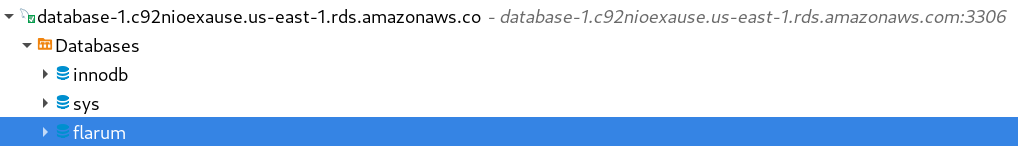
\includegraphics[frame,width=\linewidth]{img/db6.png}
\end{center}

Tras crear la base de datos, se puede pasar a realizar la creación de la máquina virtual.


\section{Mediante CLI}
Si queremos crear la instancia de RDS mediante el interfaz de línea de comandos se puede realizar a través del siguiente comando:

\begin{mycode}{Crear instancia RDS mediante CLI}{console}{}
ddd_v1_w_Hox_1818884@runweb70100:~$ aws --region us-east-1 \
    rds create-db-instance \
        --db-name mysqlcli \
        --db-instance-identifier rds-cli \
        --allocated-storage 20 \
        --db-instance-class db.t3.micro \
        --engine mysql \
        --engine-version 5.7 \
        --master-username admin \
        --master-user-password p4isQW73QW9130aS \
        --storage-encrypted \
        --no-multi-az \
        --backup-retention-period 10 \
        --preferred-backup-window 03:00-03:30 \
        --vpc-security-group-ids sg-03172af1cf7d57f66
\end{mycode}


\chapter{EC2 y despliegue de aplicación}
\textbf{EC2}, o \textit{Elastic Compute Cloud}, es la capa de negocio de Amazon que nos permite crear máquinas virtuales dentro de su sistema \textit{cloud}.

\section{Creación de la máquina virtual}
Para realizar el despliegue se va a necesitar una instancia EC2 con las siguientes características:
\begin{itemize}
    \item Tipo: \textbf{t2.micro}
    \item Arquitectura 64bits (x86)
    \item Sistema Operativo Amazon Linux 2
    \item Volumen raiz 10GiB SSD (gp2)
    \item Volumen adicional EBS de 5 GiB
\end{itemize}

Para crear la instancia debemos ir al interfaz web, buscar la sección \textbf{EC2} y darle al botón 
\includegraphics[width=0.2\linewidth]{img/boton.png} que nos abrirá el asistente para seleccionar las opciones descritas.

Durante el asistente se ha configurado el grupo de seguridad para permitir el acceso por SSH, al puerto 80 y al 443 desde mi IP personal. En apartados posteriores se detallarán más opciones acerca de los grupos de seguridad.

{
\begin{minipage}{0.6\linewidth}
    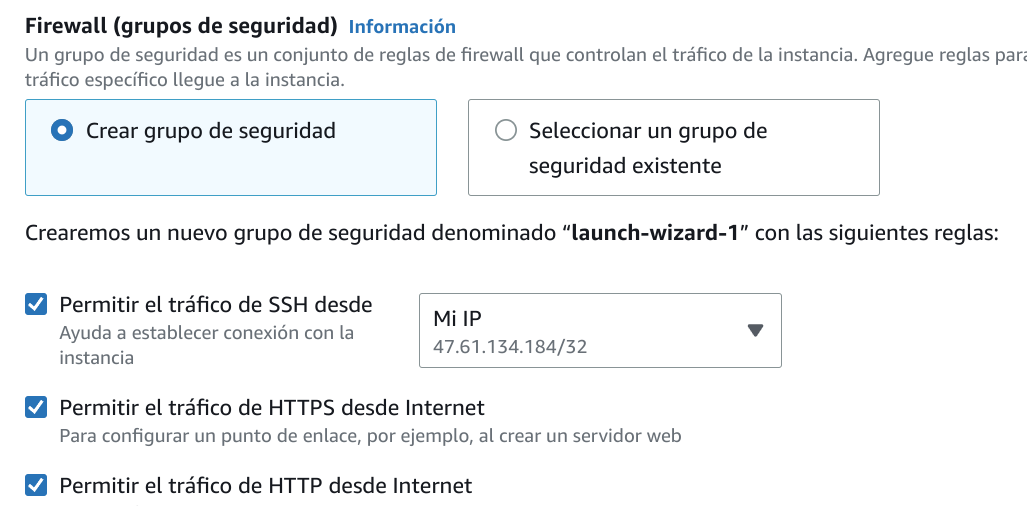
\includegraphics[frame,width=\linewidth]{img/seguridad.png}
\end{minipage}
\hfill
\begin{minipage}{0.35\linewidth}
    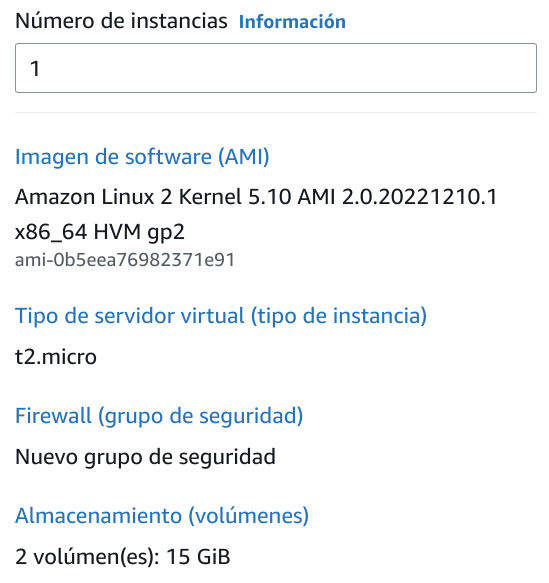
\includegraphics[frame,width=\linewidth]{img/resumen.png}
\end{minipage}
}

Tras asegurar que las opciones elegidas son las correctas, se confirma la creación de la instancia y nos aparecerá la nueva instancia en el panel principal de EC2:

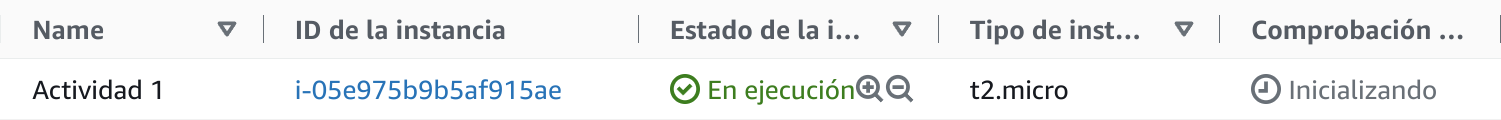
\includegraphics[frame,width=\linewidth]{img/estado.png}

\subsection{Mediante CLI}
Si queremos realizar la creación de la máquina virtual a través del interfaz de consola \textbf{aws}, deberíamos ejecutar el siguiente comando:

\begin{mycode}{Crear instancia EC2 mediante CLI}{console}{}
ddd_v1_w_Hox_1818884@runweb70100:~$ aws --region us-east-1 \
  ec2 run-instances \
    --instance-type t2.micro \
    --key-name vockey \
    --image-id ami-0b5eea76982371e91 \
    --block-device-mappings \
      '[{"DeviceName":"/dev/xvda","Ebs":{"VolumeSize":10}},
      {"DeviceName":"/dev/xvdb","Ebs":{"VolumeSize":5}}]' \
    --security-group-ids sg-0d13061c1e89dec15
\end{mycode}

La sección del parámetro “\textbf{block-device-mappings}” se podría pasar a un fichero \textbf{JSON} externo en lugar de ponerlo en el comando.

\section{Configuración previa}

Para conectarnos a la instancia se ha obtenido la \textbf{clave SSH} que otorga AWS, ya que el acceso por usuario+contraseña está deshabilitado por defecto. Para realizar el acceso se ha usado el siguiente comando:

\begin{mycode}{Acceso SSH a la instancia}{console}{}
ruben@vega:~$ ssh -i labsuser.pem ec2-user@44.211.145.168
\end{mycode}


\subsection{Creación del sistema de ficheros}
Dado que se ha añadido un segundo volumen de 5GiB a la instancia, tenemos que hacer que este sea accesible. Este nuevo volumen está situado en la ruta Linux \configfile{/dev/xvdb}

Por defecto no está formateado, por lo que debemos realizar:
\begin{itemize}
    \item Crear partición a través del comando \commandbox{fdisk}. Usaremos todo el volumen.
    \item Crear sistema de ficheros EXT-4 con el comando \commandbox{mkfs.ext4}
    \item Modificar el fichero \configfile{/etc/fstab} para que la nueva partición se monte en \configdir{/data} en caso de que la instancia se reinicie:
    \begin{mycode}{Contenido de /etc/fstab}{console}{{\footnotesize }}
UUID=a6741dbd-5f1a-4fab-8ea1-629052b08877 /data ext4 defaults,noatime 0 0
\end{mycode}
    Se podría haber utilizado \configfile{/dev/xvdb1} en lugar del UUID, pero así nos aseguramos que no existe confusión con el posible cambio de orden de los volúmenes.
\end{itemize}

Una vez realizado esto, y creado el directorio de destino, con el comando \commandbox{mount -a} se montará el nuevo volumen, quedando:

\begin{mycode}{Titulo}{console}{}
[root@ip-172-31-81-57 ec2-user]# df -h
S.ficheros     Tamaño Usados  Disp Uso% Montado en
devtmpfs         474M      0  474M   0% /dev
tmpfs            483M      0  483M   0% /dev/shm
tmpfs            483M   416K  482M   1% /run
tmpfs            483M      0  483M   0% /sys/fs/cgroup
/dev/xvda1        10G   1,6G  8,5G  16% /
tmpfs             97M      0   97M   0% /run/user/1000
/dev/xvdb1       4,8G    24K  4,6G   1% /data
\end{mycode}


\subsection{Instalación de dependencias}
La aplicación a desplegar, \href{https://flarum.org/}{Flarum}, es un desarrollo creado con el \textit{framework} \href{https://laravel.com/}{Laravel}, por lo que es un desarrollo web que requiere de las siguientes dependencias:

\begin{itemize}
    \item Servidor web Apache o Nginx
    \item PHP 7.4 o superior (con las extensiones: curl, dom, fileinfo, gd, json, mbstring, openssl, pdo\_mysql, tokenizer, zip)
    \item Base de datos MySQL 5.6 o superior
\end{itemize}

Para la gestión de la base de datos lo haremos mediante \textbf{RDS} que se comentará más adelante. Para realizar la instalación de Apache lo haremos mediante los repositorios de la distribución:

\begin{mycode}{Instalación y activación de Apache}{console}{}
[root@ip-172-31-81-57 ec2-user]# yum install apache2
[root@ip-172-31-81-57 ec2-user]# systemctl enable httpd
[root@ip-172-31-81-57 ec2-user]# systemctl start httpd
\end{mycode}

Se ha decidido utilizar la versión 8.0 de \href{https://www.php.net/}{PHP} y realizar la instalación a través de los repositorios “extra” de Amazon:

\begin{mycode}{Instalación de PHP y las dependencias necesarias}{console}{{\small }}
[root@ip-172-31-81-57 ec2-user]# amazon-linux-extras install php8.0
[root@ip-172-31-81-57 ec2-user]# yum install php-mbstring php-dom php-gd
\end{mycode}


\section{Instalación de la aplicación}

Para realizar la instalación de la aplicación Flarum se ha seguido la \href{https://docs.flarum.org/install#installing}{guía de instalación}, por lo que se usará \href{https://getcomposer.org/}{Composer} para la descarga del código.

\begin{mycode}{Descarga e instalación de Composer}{console}{{\scriptsize }}
[root@ip-172-31-81-57]# php -r "copy('https://getcomposer.org/installer', 'composer-setup.php');"
[root@ip-172-31-81-57]# php composer-setup.php --install-dir=/bin --filename=composer
\end{mycode}


La instalación utilizará la ruta \configdir{/data/www} donde se alojará la aplicación.

\begin{mycode}{Descarga e instalación de Composer}{console}{{\small }}
[root@ip-172-31-81-57 ec2-user]# mkdir /data/www
[root@ip-172-31-81-57 ec2-user]# cd /data/www/
[root@ip-172-31-81-57 www]# composer create-project flarum/flarum .
\end{mycode}

Y tras esto hay que añadir la configuración correspondiente del VirtualHost en el fichero \configfile{/etc/httpd/conf/httpd.conf} y reiniciar el servicio.

\begin{mycode}{Configuración Apache}{ApacheConf}{}
<VirtualHost *:80>
  DocumentRoot "/data/www/public"
  ServerName actividad1-08masw.universidadviu.com
  DirectoryIndex index.php
  <Directory "/data/www/public">
    AllowOverride All
    Options Indexes FollowSymLinks
    Require all granted
  </Directory>
</VirtualHost>
\end{mycode}

Tal como se puede ver en la configuración, se ha añadido un dominio a la configuración, \textbf{actividad1-08masw.universidadviu.com}, por lo que para acceder deberemos modificar nuestro fichero \configfile{/etc/hosts}. Tras esto, en el navegador podremos ver cómo aparece la web de configuración de Flarum:

\begin{center}
    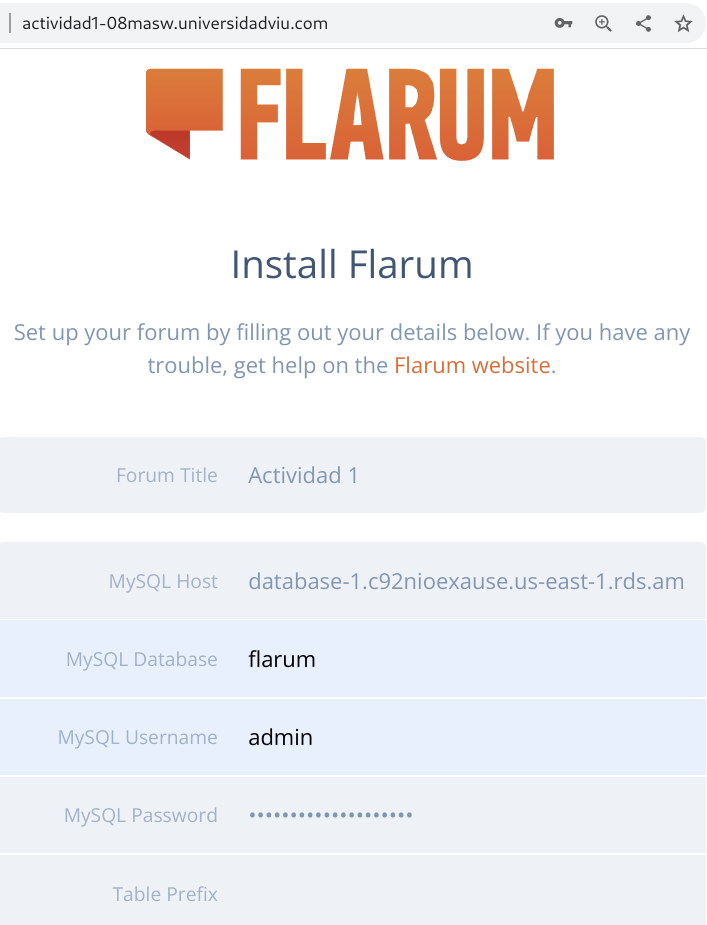
\includegraphics[frame,width=0.5\linewidth]{img/installer.png}
\end{center}

Se ha introducido la configuración obtenida de la creación de la base de datos RDS, y tras esto ya tenemos acceso a la aplicación. Para comprobar su correcto funcionamiento se han creado dos posts de pruebas:

\begin{center}
    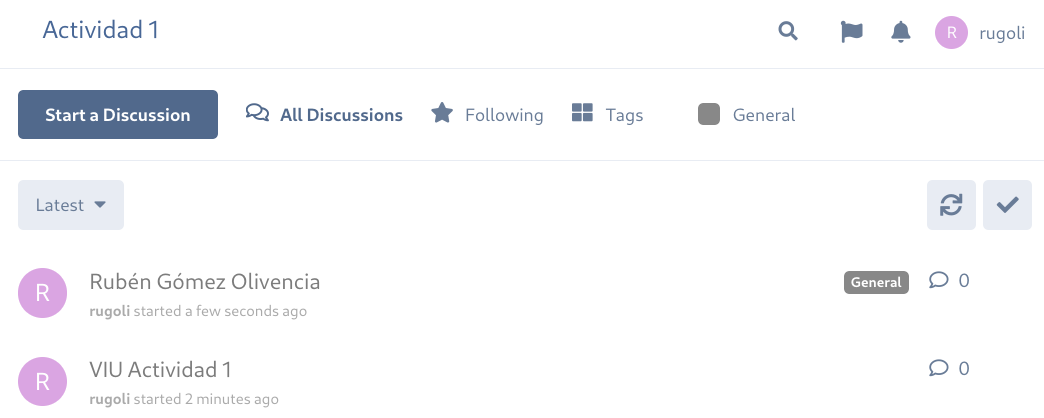
\includegraphics[frame,width=0.9\linewidth]{img/flarum.png}
\end{center}

% TODO: comentar la configuración



\chapter{Grupos de seguridad}
Para facilitar la seguridad de las instancias existen los \textbf{grupos de seguridad}. Con ellos, podemos crear reglas de entrada y reglas de salida, para distintos puertos y protocolos que nos interese filtrar.

Podemos crear grupos de seguridad que posteriormente se asignan a instancias, y de esta manera centralizar la seguridad. En caso de necesitar añadir o quitar IPs o protocolos, al modificar el grupo de seguridad se aplicará a las instancias que hagan uso de dicho grupo.

A modo de pruebas se ha creado el grupo de seguridad “Servidores Web”, que cuenta con las siguientes reglas de entrada:
\begin{itemize}
    \item Aceptar cualquier conexión al puerto TCP 80 (conexión HTTP).
    \item Aceptar cualquier conexión al puerto TCP 443 (conexión HTTPS).
    \item Aceptar conexiones al puerto 22 (SSH) sólo desde la IP 83.138.41.161 (administrador remoto).
    \item Aceptar conexiones al puerto 22 (SSH) sólo desde la IP 47.61.134.184 (administrador remoto).
\end{itemize}

\begin{center}
    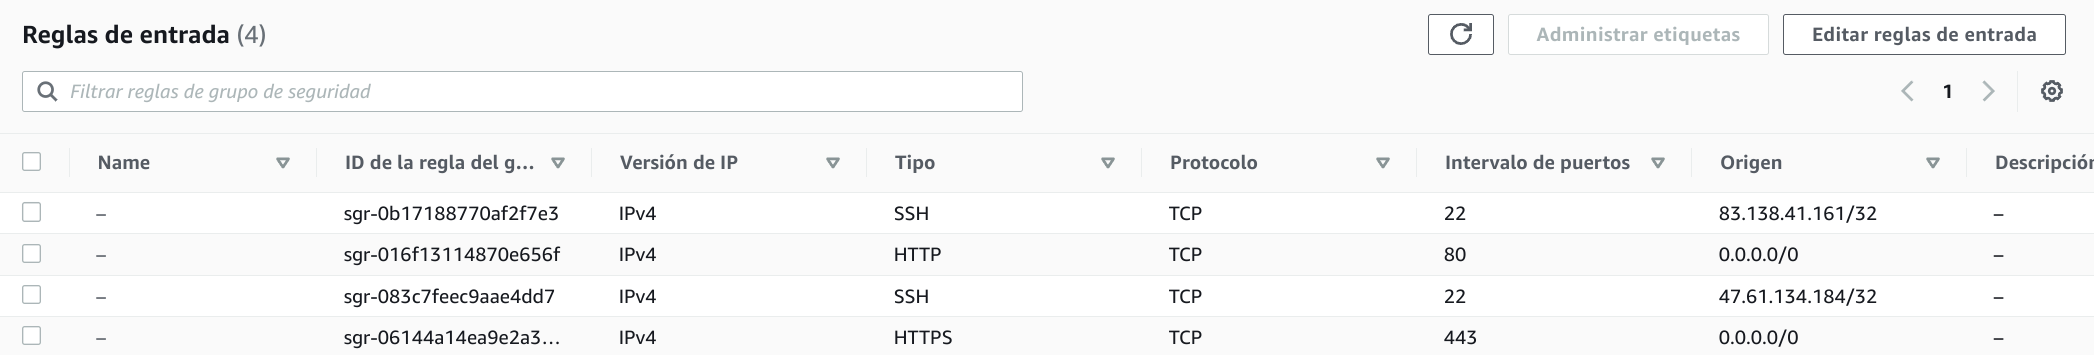
\includegraphics[frame,width=\linewidth]{img/grupos.png}
\end{center}

Tras crear el grupo lo que tenemos que hacer es asignarlo a la instancia creada previamente:

\begin{center}
    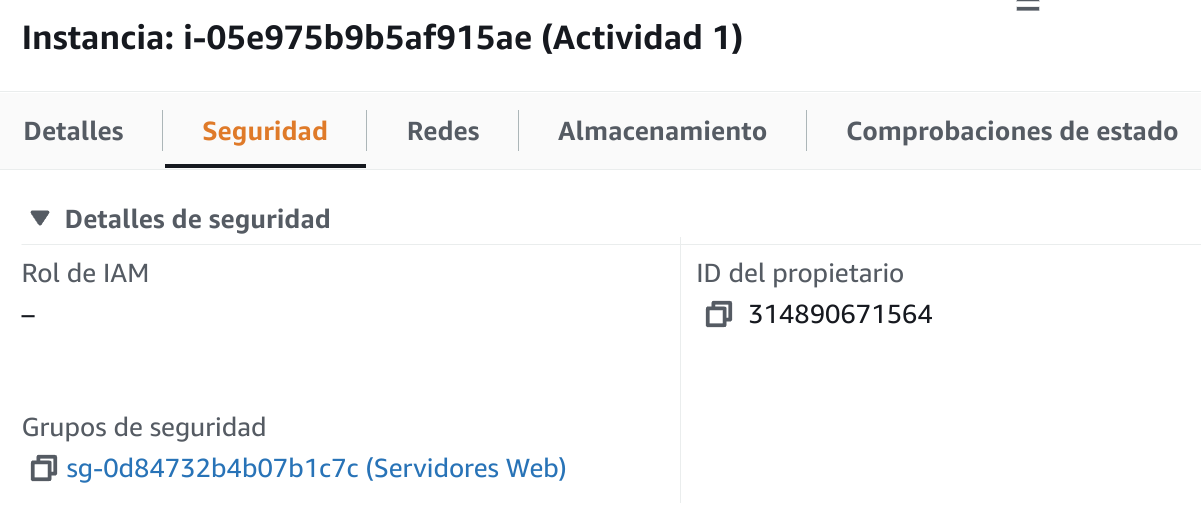
\includegraphics[frame,width=0.7\linewidth]{img/grupos2.png}
\end{center}

También podremos realizar la asignación en el momento en el que se crea una instancia nueva, de esta manera nos aseguramos que ya desde el momento de la creación sólo se tiene acceso desde las IPs que nos interese.

\section{Mediante CLI}

Los grupos de seguridad también se pueden crear a través de línea de comandos, pero es necesario hacerlo en varios pasos. Primero se crea el “\textit{security group}” y después se le añaden las reglas.

Se va a crear el ejemplo expuesto previamente a través del CLI, y para añdir las reglas es necesario conocer el \textbf{GroupID} que devuelve el primer comando:

\begin{mycode}{Crear \textit{security group} y añadirle reglas}{console}{}
ddd_v1_w_Hox_1818884@runweb70100:~$ aws --region us-east-1 \
  ec2 create-security-group \
    --group-name servidores-web \
    --description “para servidores web”

ddd_v1_w_Hox_1818884@runweb70100:~$ aws --region us-east-1 \
  ec2 authorize-security-group-ingress \
  --group-id sg-0d13061c1e89dec15 \
  --protocol tcp --port 22 \
  --cidr 83.138.41.161/32

ddd_v1_w_Hox_1818884@runweb70100:~$ aws --region us-east-1 \
  ec2 authorize-security-group-ingress \
    --group-id sg-0d13061c1e89dec15 \
    --protocol tcp --port 22 \
    --cidr 47.61.134.184/32


ddd_v1_w_Hox_1818884@runweb70100:~$ aws --region us-east-1 \
  ec2 authorize-security-group-ingress \
    --group-id sg-0d13061c1e89dec15 \
    --protocol tcp --port 80 \
    --cidr 0.0.0.0/0

ddd_v1_w_Hox_1818884@runweb70100:~$ aws --region us-east-1 \
  ec2 authorize-security-group-ingress \
    --group-id sg-0d13061c1e89dec15 \
    --protocol tcp --port 443 \
    --cidr 0.0.0.0/0
\end{mycode}

Es importante darse cuenta que a la hora de crear mediante línea de comandos la instancia EC2 y la RDS se han añadido distintos IDs de \textit{security-groups}, que lógicamente deben existir previamente.


\chapter{IP elástica}

Por cómo funciona las instancias EC2, la asignación de IPs públicas es temporal, por lo que en el momento en el que una instancia se para, al volverla a levantar no obtendrá la misma IP pública.

Para evitar esto están las \textbf{IP elásticas}, que se pueden crear desde el menú de EC2, en “\textbf{Red y Seguridad > Direcciones IP elásticas}”. Desde este apartado podremos realizar la solicitud de una IP elástica, pero que no se podrá utilizar mientras no sea asignada a una instancia.

Es por ello que hay que seleccionar la IP elástica recién creada, y a través del menú “Acciones” pulsar la opción “Asociar la dirección IP elástica. De esta manera podremos asociarla a la instancia que nos interese. En nuestro caso a la instancia creada previamente:

\begin{center}
    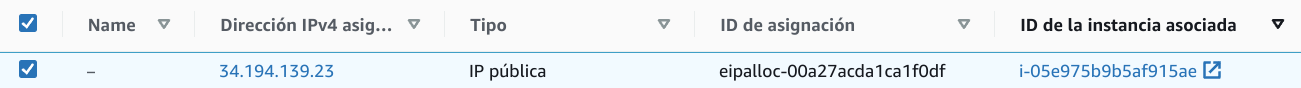
\includegraphics[frame,width=\linewidth]{img/ip_elastica.png}
\end{center}

De esta manera, aunque ahora la instancia se pare, no pasará nada, ya que al volver a levantarse mantendrá la IP.

Es importante acordarse que hemos modificado el fichero \configfile{/etc/hosts}, por lo que ahora deberemos reflejar la nueva IP para poder acceder al dominio de la aplicación. Lo mismo para el acceso por SSH.


\chapter{Bucket S3}

Otro de los servicios que ofrece AWS es \textbf{S3} (de “\textit{Simple Storage Service}”), donde podremos almacenar objetos a través de un interfaz REST (o a través de los SDK). Se han elegido las siguientes opciones al crear un bucket:

%Para crear el bucket se ha ido al apartado de S3, donde aparece el botón de “Crear bucket”, donde se han elegido las siguientes opciones:

\begin{center}
    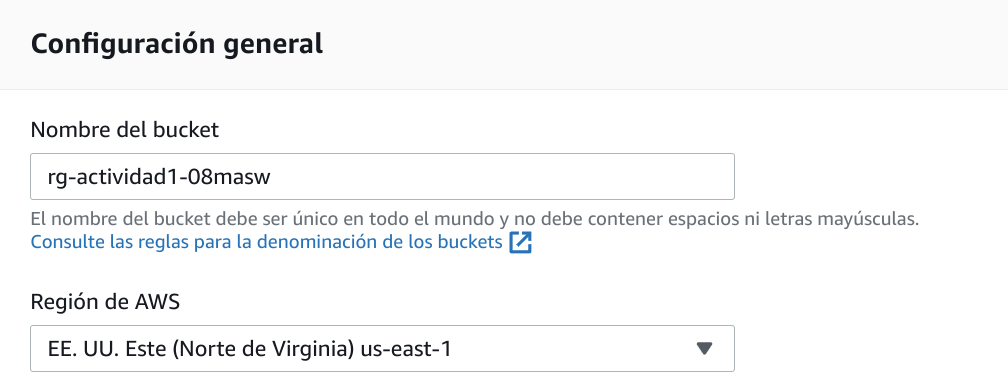
\includegraphics[width=0.8\linewidth]{img/s31.png}
%    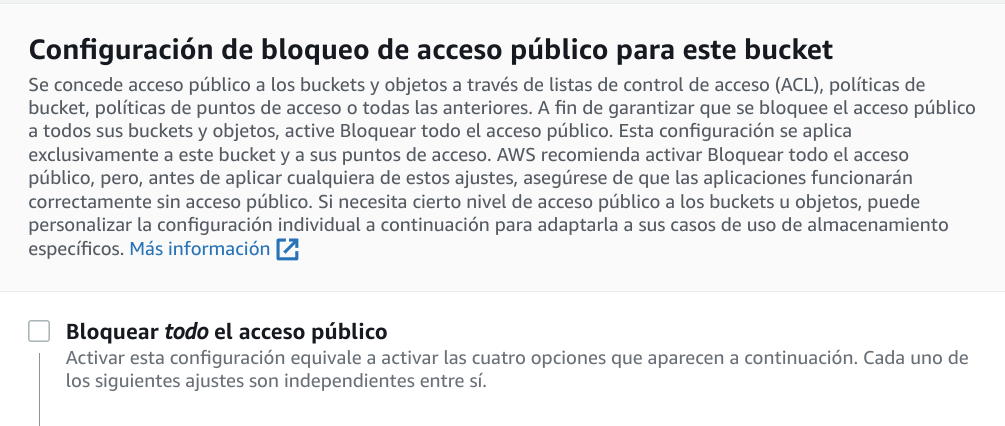
\includegraphics[width=0.8\linewidth]{img/s32.png}
    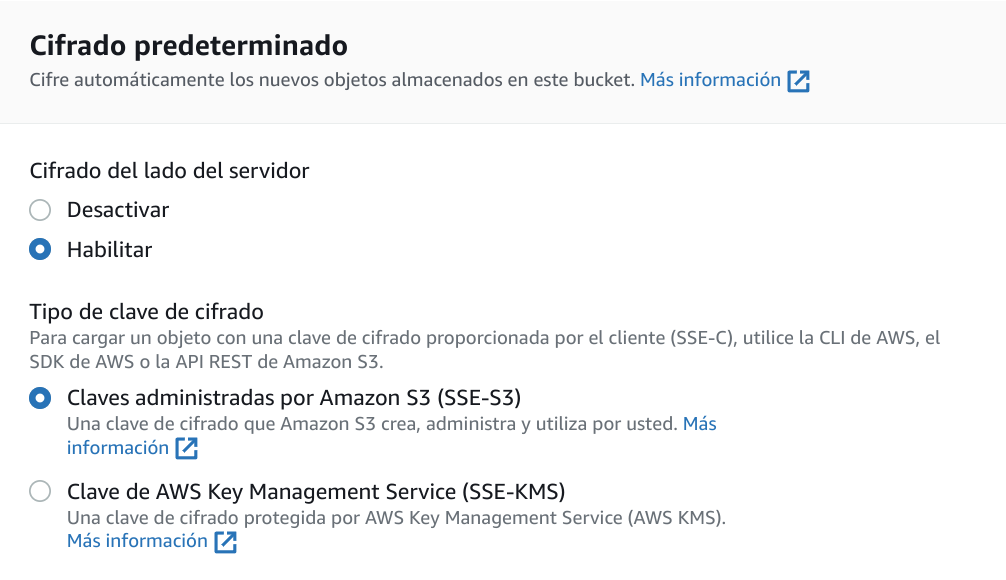
\includegraphics[width=0.8\linewidth]{img/s33.png}
\end{center}

Si queremos crear el bucket desde la línea de comandos se puede hacer con el siguiente comando:

\begin{mycode}{Crear bucket S3}{console}{{\small }}
ddd_v1_w_Hox_1818884@runweb69965:~$ aws s3 mb s3://rg-actividad1-08masw
make_bucket: rg-actividad1-08masw
\end{mycode}


Una vez creado, se pueden añadir ficheros a través del interfaz web o desde el la consola de AWS, ejecutando lo siguiente para subir una imagen al bucket:

\begin{mycode}{Subir fichero SVG al bucket S3}{console}{{\scriptsize }}
ddd_v1_w_Hox_1818884@runweb69965:~$ aws s3 cp logo.svg s3://rg-actividad1-08masw/logo.svg
upload: ./logo.svg to s3://rg-actividad1-08masw/logo.svg
\end{mycode}

Los objetos subidos pueden ser públicos a través de distintas ACLs que se pueden crear. A continuación dos enlaces con ficheros de pruebas subidos:

% TODO: poner enlaces
\begin{itemize}
    \item
    \item
\end{itemize}


\chapter{Costes estimados}
Debido a todas las opciones con las que cuenta AWS, puede resultar confuso el precio final que se termina pagando. Es por eso que Amazon cuenta con el \href{https://calculator.aws/}{Amazon Pricing Calculator} para poder estimar los costes.

Teniendo en cuenta las siguientes características:

\begin{itemize}
    \item Instancias bajo demanda sin reserva.
    \item Estimación tráfico de entrada servidor web de 15 GB/mes
    \item Estimación tráfico de salida servidor web de 30GB/mes.
    \item Tráfico de salida del servicio de S3 10GB/mes.
\end{itemize}

En la siguiente tabla se van a comparar los costes estimados por mes para dos regiones (España y USA-Virginia) teniendo en cuenta todo lo visto hasta ahora:

\begin{yukitblrcol}{X[3]X[1]X[1]}
        & España & N. Virginia \\
    Instancia EC2 t2.micro Linux, 15GB EBS gp2, con tráfico estimado
        & \$9,97/mes \textbf{*} & \$9,97/mes \\
    IP elástica
        & \$0/mes & \$0/mes \\
    Base de datos RDS MySQL db.t3.micro, single-AZ, sin proxy, almacenamiento 20GB, 40GB copias de seguridad \textbf{**}
        & \$20,54/mes & \$18,51/mes \\
    Bucket S3, 1GB de almacenamiento, con tráfico estimado de salida \textbf{***}
        & \$0,02/mes & \$0,02/mes \\
\end{yukitblrcol}
\begin{itemize}
    \item[*] En España sólo se puede coger una instancia \textbf{t3}.micro, que tiene más CPU.
    \item[**] La estimación para los backups al comienzo del proyecto podría ser menor, pero si se pretende llegar a los 20GB de espacio, para una retención de 10 días los 40GB se quedarán cortos.
    \item[***] Si el número de peticiones está por debajo de 100.000 el precio no varía. Tampoco se tiene en cuenta el cargar los datos iniciales.
\end{itemize}

Tal como se ha podido comprobar en la tabla, los precios son similares en ambas regiones. En el caso de la instancia EC2, por el mismo precio obtenemos una máquina virtual mejor, mientras que la instancia de base de datos es un poco más cara.

De todas formas, también hay que tener en cuenta la latencia de acceso a las instancias. En el mejor de los casos el acceso a Virginia es dos veces más lento que a España, y en el peor hasta 6 veces. Para comprobarlo se pueden utilizar distintas herramientas que comprueban la latencia (\href{https://www.cloudping.info/}{enlace 1}, \href{https://www.awsspeedtest.com/latency}{enlace 2}).

\chapter{Conclusiones}

La gestión de

\end{document}
